\documentclass[11pt,letterpaper]{article}
\usepackage[margin=1in]{geometry}
\usepackage{fontspec}
\usepackage{microtype,booktabs,graphicx,amsmath,longtable,array,adjustbox,float}
\usepackage[round,authoryear]{natbib}
\usepackage[font=small,labelfont=bf]{caption}
\usepackage[hidelinks]{hyperref}
\usepackage{xurl,setspace}
\setstretch{1.15}
\setlength{\emergencystretch}{2em}
\graphicspath{{../figs/}}
% Generated by scripts/tables.R; do not edit.
\newcommand{\Retractions}{67,440}
\newcommand{\Frame}{9,555}
\newcommand{\Resolved}{8,963}
\newcommand{\Matched}{8,627}
\newcommand{\Unmatched}{323}
\newcommand{\Stacks}{8,627}
\newcommand{\Comparison}{23,528}
\newcommand{\Controls}{26,138}
\newcommand{\MainPercent}{-62.1}
\newcommand{\MainLower}{-62.9}
\newcommand{\MainUpper}{-61.2}
\newcommand{\MainReduction}{62.1}
\newcommand{\FivePercent}{-65.8}
\newcommand{\FiveLower}{-66.6}
\newcommand{\FiveUpper}{-65.0}
\newcommand{\JournalYearPercent}{-63.1}
\newcommand{\JournalYearLower}{-63.7}
\newcommand{\JournalYearUpper}{-62.4}
\newcommand{\JournalYearComparison}{81,796}
\newcommand{\JournalYearMinusThree}{8.3}
\newcommand{\JournalYearMinusTwo}{6.4}
\newcommand{\AdditiveEstimate}{-2.45}
\newcommand{\AdditiveLower}{-2.55}
\newcommand{\AdditiveUpper}{-2.36}
\newcommand{\PretrendP}{< 0.001}
\newcommand{\EventMinusThree}{5.7}
\newcommand{\EventMinusTwo}{4.5}
\newcommand{\EventZero}{-18.6}
\newcommand{\EventOne}{-51.5}
\newcommand{\EventThree}{-70.4}
\newcommand{\EventFive}{-74.7}
\newcommand{\EventFiveLower}{-75.7}
\newcommand{\EventFiveUpper}{-73.7}
\newcommand{\RetractedMeanBefore}{4.4}
\newcommand{\RetractedMeanAfter}{1.2}
\newcommand{\ComparisonMeanBefore}{4.0}
\newcommand{\ComparisonMeanAfter}{3.4}
\newcommand{\RetractedMedianBefore}{2}
\newcommand{\RetractedMedianAfter}{0}
\newcommand{\RetractedZeroAfter}{55.7}
\newcommand{\ComparisonZeroAfter}{31.1}
\newcommand{\LegacyOpenAlexPercent}{-51.4}
\newcommand{\LegacyWosPercent}{-46.5}
\newcommand{\LegacyWosAdditive}{-1.76}
\newcommand{\LegacyWosArticles}{3,002}
\newcommand{\AckAfterPercent}{91.4}
\newcommand{\AckAfterLower}{87.3}
\newcommand{\AckAfterUpper}{94.3}
\newcommand{\AckAfterCoded}{256}
\newcommand{\AckAfterUnack}{234}
\newcommand{\AckBeforeCoded}{52}
\newcommand{\AckBeforeUnack}{52}
\newcommand{\AckBeforePercent}{100.0}
\newcommand{\PostArticles}{8,963}
\newcommand{\PostCitations}{305,552}
\newcommand{\PostAfter}{82,013}
\newcommand{\PostAfterShare}{26.8}
\newcommand{\PostCitedShare}{80.4}
\newcommand{\PostMedianAfter}{3}
\newcommand{\PostMeanAfter}{9.2}
\newcommand{\PostCitedAtFive}{39.3}
\newcommand{\PostMeanAtFive}{1.1}
\newcommand{\PostArticlesAtFive}{5,821}
\newcommand{\PostCitedAtEight}{31.6}
\newcommand{\MeanLag}{5.0}
\newcommand{\MedianLag}{4}
\newcommand{\LagFourPlusPercent}{55.5}
\newcommand{\HetMisconduct}{-64.2}
\newcommand{\HetDuplication}{-57.8}
\newcommand{\HetError}{-64.1}
\newcommand{\HetOther}{-47.4}
\newcommand{\HetReasonP}{< 0.001}
\newcommand{\HetFieldP}{< 0.001}
\newcommand{\HetFieldMin}{-67.7}
\newcommand{\HetFieldMax}{-56.0}
\newcommand{\HetTercileP}{= 0.075}
\newcommand{\HetLagTwo}{-67.1}
\newcommand{\HetLagSixPlus}{-56.0}
\newcommand{\HetLagP}{< 0.001}
\newcommand{\HetPriorYes}{-66.7}
\newcommand{\HetPriorNo}{-61.7}
\newcommand{\HetPriorP}{= 0.003}
\newcommand{\LooMin}{-63.0}
\newcommand{\LooMax}{-60.4}
\newcommand{\JournalClusteredLower}{-63.7}
\newcommand{\JournalClusteredUpper}{-60.4}
\newcommand{\MisconductShare}{41.0}
\newcommand{\DuplicationShare}{32.8}
\newcommand{\ErrorShare}{18.9}
\newcommand{\WosOpenAlexRatio}{1.10}
\newcommand{\WosExactShare}{50.0}
\newcommand{\WosWithinOneShare}{78.2}
\newcommand{\WosArticleYears}{19,351}
\newcommand{\WosOverlap}{1,284}
\newcommand{\WosNoticeYearAgreement}{94.2}
\newcommand{\HonestAvailable}{1}
\newcommand{\SdidEstimate}{-2.27}
\newcommand{\SdidLower}{-2.41}
\newcommand{\SdidUpper}{-2.14}
\newcommand{\SdidCohorts}{18}
\newcommand{\SdidTreated}{6,720}
\newcommand{\HonestBreakdown}{2.0}
\newcommand{\HonestMaxMbar}{2.0}
\newcommand{\HonestLowerAtMax}{-70.4}
\newcommand{\HonestUpperAtMax}{-52.3}
\newcommand{\HonestMaxPreChange}{4.5}

\title{Propagation of Error: Citations to Retracted Research}
\author{Ken Cor \and Gaurav Sood}
\date{October 2026}
\hypersetup{pdfauthor={Ken Cor and Gaurav Sood},pdftitle={Propagation of Error: Citations to Retracted Research}}
\widowpenalty=10000
\clubpenalty=10000
\begin{document}
\maketitle
\begin{abstract}
\noindent A retraction is the strongest public signal that an article should not be relied on. We estimate how citations to retracted articles change after retraction by comparing each of \Stacks{} retracted research articles, published 2000--2019 and retracted 2005--2022, with up to five articles from the same journal and publication year matched on pre-retraction citations. Citation histories through 2025 come from OpenAlex for retracted and comparison articles alike. In the three complete years after the retraction year, citations to retracted articles were \MainPercent\% (95\% interval [\MainLower, \MainUpper]\%) relative to the path of their comparison articles, and the gap widens with time from retraction. Retracted articles continue to be cited: \PostAfterShare\% of all citations to these articles arrived after the retraction year, five years on \PostCitedAtFive\% of the articles observed that long were still cited, and in a 2016 sample of citing passages \AckAfterUnack{} of \AckAfterCoded{} post-retraction citations recorded no concern with the cited article. Retracted articles were slipping slightly relative to their matches before the notice; sensitivity bounds that allow that slippage to continue at twice its pace leave most of the decline in place. The earlier draft of this paper, which had no comparison group and omitted every year in which an article received no citations, understated the decline.
\end{abstract}
\vspace{1em}
\noindent\textbf{Keywords:} retractions; citation analysis; scientific self-correction; difference-in-differences; synthetic control

\newpage
\section{Introduction}
Citations transmit trust. Unless the citing author says otherwise, a citation tells the reader that the cited data, method or result can be used. When the cited article has been retracted, that signal is false, and the error propagates: a reader may build on the point, cite the retracted article for it in turn, or carry it into a meta-analysis. The 2005 \textit{Cancer Research} report that stem cells spontaneously transform into cancerous cells in culture was retracted in 2010 after the result failed to replicate and cross-contamination emerged as the likely cause \citep{rubio2005spontaneous,de2010retraction}; it was cited more than three hundred times after that, mostly as evidence \citep{firinci2011mesenchymal,kosaka2012therapeutic,chang2013safety}.

This paper asks two questions. How much does a retraction reduce citations to the retracted article, relative to what the article would otherwise have received? And when retracted articles are cited afterward, how often does the citing passage record the retraction?

The first question needs a comparison. Citations to any article rise for a few years after publication and then fall, and most retractions happen two to three years after publication, near the peak. A before-and-after comparison therefore confounds the retraction with the ordinary life cycle of citations. We follow the matched-control design of \citet{furman2012} and \citet{azoulay2015}: each retracted article is paired with articles from the same journal and publication year with similar citations before the retraction, and the outcome is the retracted article's proportional change relative to its own comparison articles. We estimate it on every Retraction Watch retraction of a research article that meets our frame rules (\Frame{} articles), with citation histories through 2025 from OpenAlex measured identically for both arms, and we pre-registered the rules in the repository before estimating anything.

The second question is answered with a hand-coded sample of citing passages collected in 2016 for the earlier version of this paper, which we retain as historical coding. The companion paper examines the same questions for methodological critiques that do not lead to retraction \citep{cor2026}.

\section{Prior evidence}
Three facts about retractions are well established. Retractions have grown faster than the literature \citep{steen2011retractions,grieneisen2012comprehensive}. Most are for misconduct or serious error rather than honest mistakes \citep{bozzo2017retractions,singh2014comprehensive}. And retracted articles keep being cited, usually without any mention of the retraction, in samples spanning biomedicine, radiation oncology and case reports \citep{pfeifer1990continued,budd1998phenomena,bar2017post,hamilton2019continued,luwel2018schon,hsiao2021}. Citing authors who are unfamiliar with a field or rely on prominent journals are more likely to cite retracted work \citep{woo2024}.

The size of the citation penalty is less settled. With matched controls, \citet{furman2012} find that citations to retracted biomedical articles fall by more than half, \citet{lu2013} find a penalty that spreads to the retracted authors' other work, and \citet{azoulay2015} find a smaller penalty on related but unretracted articles that is larger after misconduct. Our contribution is scale and openness: a census of eligible retractions across fields rather than a biomedical sample, open data so the result can be rebuilt, and a design that reports its own pre-trends, heterogeneity and sensitivity.

\section{Data}
\subsection{Retracted articles}
The retraction registry is the Retraction Watch database, which Crossref publishes as an open file \citep{retractionwatch2026}. Our snapshot holds \Retractions{} retraction records. We keep one record per original DOI (the earliest retraction), require the original to be a research article or clinical study published 2000--2019 and retracted 2005--2022 at least two years after publication, so that at least one complete pre-retraction year exists, and require the DOI to resolve to one OpenAlex journal article whose publication year agrees with Retraction Watch's within a year. The sample-flow table in the appendix lists every step. The frame has \Frame{} articles, of which \Resolved{} resolve. Retraction Watch's reasons are grouped literally: \MisconductShare\% carry a fabrication, manipulation, paper-mill or peer-review label, \DuplicationShare\% a plagiarism or duplication label, and \ErrorShare\% an error or unreliability label; the rest state an investigation or little else. The median article was retracted \MedianLag{} years after publication (mean \MeanLag), and \LagFourPlusPercent\% took four years or more.

\subsection{Citations}
The outcome is the number of articles and reviews citing an article in each year, from the article's publication year through 2025, from OpenAlex \citep{priem2022}. Years with no citations are zeros, not missing. Comparison articles are measured with the same query. We validated the measure against the Web of Science export used in the earlier draft: for \WosArticleYears{} article-years covering the same articles from publication through 2015, OpenAlex counts are \WosOpenAlexRatio{} times the Web of Science counts, agree exactly in \WosExactShare\% of article-years and within one citation in \WosWithinOneShare\%. For the \WosOverlap{} articles in both the 2016 sample and the frame, the Retraction Watch retraction year equals the Web of Science notice year in \WosNoticeYearAgreement\%.

\subsection{Comparison articles}
For each retracted article we draw a seeded random sample of twenty articles from the same OpenAlex journal and publication year, excluding any that OpenAlex or Retraction Watch flags, and match on two quantities measured strictly before the retraction year: the logarithm of one plus cumulative citations, and the logarithm of one plus citations in the year before retraction. Both are standardized within the pool, a candidate must be within one standard deviation on each, and the five nearest are kept with equal weight. \Matched{} retracted articles find at least one comparison article (\Controls{} distinct comparison articles); \Unmatched{} have no candidate within the caliper and are reported, not dropped. Matching uses no information from the retraction year onward, and a test in the repository perturbs post-retraction outcomes and checks that the matches do not change.

\subsection{Acknowledgment coding}
In 2016 we sampled 100 articles citing a retracted article before or in its retraction year and 275 citing one afterward, located the passages, and coded whether the citing text noted any concern with the cited article. We keep that coding as it was made; the appendix gives the full accounting.

\section{Design}
Each retracted article and its comparison articles form a stack. The main estimate is a Poisson quasi-maximum-likelihood regression of annual citations on an indicator for a retracted article in the post-retraction years, with a fixed effect for each article within its stack and for each stack and event year, so every stack supplies its own citation path and the coefficient is the retracted article's proportional change relative to its matched articles \citep{wooldridge2023,chen2024,berge2018}. The pre-period is up to three years before retraction and the post-period is years one to three after; the retraction year is reported separately because it is only partly exposed. Comparison articles receive weight one over the number of matches in their stack. Standard errors are clustered by article, because a comparison article can serve several stacks.

The dynamic version replaces the indicator with event-year interactions, with the year before retraction as the reference, which displays the pre-trend and the shape of the response. A second comparison drops the citation matching and uses every sampled article from the same journal and publication year with equal weights, the design of the earlier draft's companion analysis; it asks whether the matching step, rather than the journal-year comparison, drives the estimate. An additive version estimates the same contrast in citations per year. A synthetic difference-in-differences estimate by retraction-year cohort \citep{arkhangelsky2021} re-weights the comparison articles and the pre-years to fit the retracted articles' pre-period path, for the stacks with three complete years on each side, with whole-article bootstrap intervals. The pre-specified heterogeneity splits are reason, field, pre-retraction citation tercile, years to retraction, and a prior expression of concern. The repository's pre-analysis plan fixes all of these choices.

\section{Results}
\subsection{Citations fall after retraction and keep falling}
Figure~\ref{fig:paths} shows mean and median citations per year by years from retraction for retracted and comparison articles. Before retraction the two paths have the same shape, rising toward the year before retraction, and the retracted articles sit a little above their matches throughout: the nearest neighbours of a well-cited article among twenty sampled candidates lie mostly below it, and the fixed effects absorb that level difference. In the year before retraction the mean retracted article received \RetractedMeanBefore{} citations and the mean comparison article \ComparisonMeanBefore. Three years after retraction the means were \RetractedMeanAfter{} and \ComparisonMeanAfter. The median retracted article went from \RetractedMedianBefore{} citations to \RetractedMedianAfter, and \RetractedZeroAfter\% of retracted articles received no citations three years after retraction, against \ComparisonZeroAfter\% of comparison articles.

\begin{figure}[H]
\centering
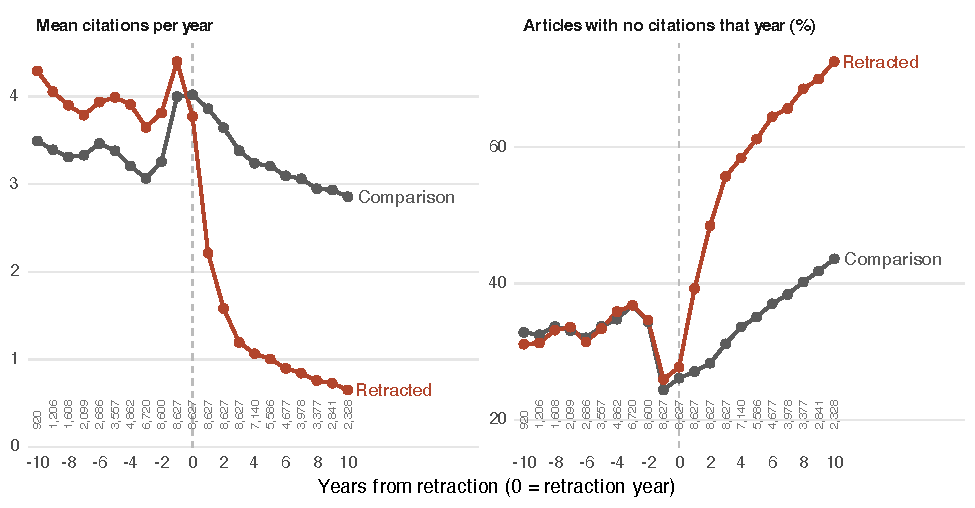
\includegraphics[width=\linewidth]{citation_paths}
\caption{Citations per year to retracted articles and their matched comparison articles, by years from retraction. Means and medians over articles, weighting each comparison article by one over the number of matches in its stack; the comparison articles come from the same journal and publication year as the retracted article and were matched on citations before the retraction year. No intervals are drawn: the panel is a census of the matched articles.}
\label{fig:paths}
\end{figure}

The main model puts the change at \MainPercent\% (95\% interval [\MainLower, \MainUpper]\%) over years one to three after retraction (Table~\ref{tab:estimates}). Extending the post-period to five years gives \FivePercent\% [\FiveLower, \FiveUpper]\%. In citations per year, the additive model gives a change of \AdditiveEstimate{} [\AdditiveLower, \AdditiveUpper] citations per year. Replacing the matched articles with all \JournalYearComparison{} sampled articles from the same journal and publication year, unmatched and equally weighted, gives \JournalYearPercent\% [\JournalYearLower, \JournalYearUpper]\%: the journal-year comparison carries the result, and the matching step changes it little. The event-year estimates in Figure~\ref{fig:event} show the time path: \EventMinusThree\% and \EventMinusTwo\% in the two years before the reference year; \EventZero\% in the retraction year; \EventOne\% one year after; and \EventFive\% [\EventFiveLower, \EventFiveUpper]\% five years after.

The pre-period coefficients are small but not zero. The ratio of retracted to comparison citations was higher three and two years before retraction than in the year before, so the retracted articles were already slipping relative to their matches, and a joint test of the two pre-period coefficients rejects equality ($p \PretrendP$). Without matching the pre-period gap is larger (\JournalYearMinusThree\% and \JournalYearMinusTwo\%), which is what the matching on pre-retraction citations is for. The sample is large enough to detect a gap of a few percent, and this one is in the direction of the later decline: whatever makes an article retractable may already cost it citations before the notice. We therefore report the sensitivity bounds of \citet{rambachan2023}, which allow the post-retraction gap to depart from the comparison path by a multiple of the largest year-to-year movement seen before retraction (\HonestMaxPreChange\%). Allowing departures up to \HonestMaxMbar{} times that movement, the three-year change stays between \HonestLowerAtMax\% and \HonestUpperAtMax\%. A pre-trend of the size we observe cannot produce a decline of the size we estimate.

\begin{figure}[H]
\centering
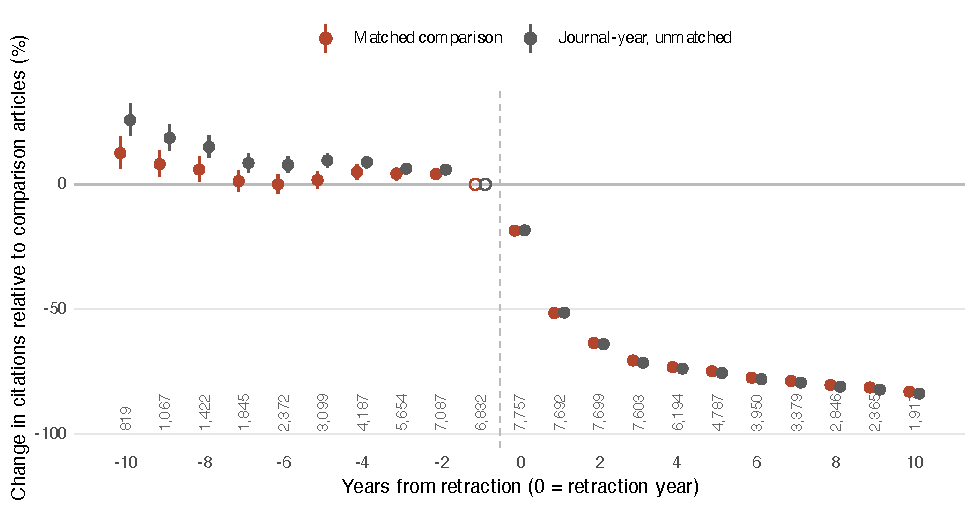
\includegraphics[width=\linewidth]{event_study}
\caption{Change in citations to retracted articles relative to comparison articles, by years from retraction: matched comparison articles (dark) and all sampled articles from the same journal and publication year, unmatched (grey). Poisson coefficients with article-within-stack and stack-by-year fixed effects, converted to percent; the year before retraction is the reference (open circles). Bars are 95\% intervals from standard errors clustered by article.}
\label{fig:event}
\end{figure}

\begin{table}[H]
\centering
\caption{Change in citations to retracted articles relative to matched comparison articles. PPML rows report the percent change implied by the Poisson coefficient; the OLS row reports citations per year. Intervals are 95\%, clustered by article.}
\label{tab:estimates}
\adjustbox{max width=\linewidth}{\begin{tabular}{p{5.2cm}lrrr}
\toprule
Specification & Model & Retracted / comparison & Estimate & 95\% interval \\
\midrule
Main: matched stacks, years +1 to +3 & PPML & 159 / 707 & -55.6\% & [-61.3, -49.0]\% \\
Years +1 to +5 & PPML & 161 / 717 & -59.7\% & [-64.3, -54.6]\% \\
Year +1 only & PPML & 150 / 663 & -41.1\% & [-48.1, -33.3]\% \\
Pre-period -1 only & PPML & 153 / 697 & -57.5\% & [-62.7, -51.7]\% \\
Additive (OLS) & OLS & 175 / 777 & -2.10 & [-2.69, -1.51] \\
Nearest match only & PPML & 154 / 154 & -53.1\% & [-60.8, -43.8]\% \\
\bottomrule
\end{tabular}
}
\end{table}

\subsection{Synthetic difference-in-differences}
Within each retraction-year cohort, the synthetic difference-in-differences estimate re-weights the comparison articles to match the retracted articles' pre-period path. Pooled by inverse variance over \SdidCohorts{} cohorts and \SdidTreated{} retracted articles with three complete years on each side, the change is \SdidEstimate{} citations per year (95\% interval [\SdidLower, \SdidUpper]); the cohort estimates are in the appendix.

\subsection{Who is penalized}
Table~\ref{tab:heterogeneity} reports the main contrast by reason for retraction, field, pre-retraction citation tercile, years to retraction, and a prior expression of concern, with a joint test of equality within each split. The decline is large in every group and differs by group. Articles retracted for misconduct (\HetMisconduct\%) or error (\HetError\%) lose more than articles retracted for plagiarism or duplication (\HetDuplication\%), and articles whose notice states no clear reason lose least (\HetOther\%; joint test $p \HetReasonP$). Across fields the change runs from \HetFieldMin\% to \HetFieldMax\% ($p \HetFieldP$). Articles retracted sooner lose more: \HetLagTwo\% when retracted two years after publication against \HetLagSixPlus\% after six or more years ($p \HetLagP$), consistent with a penalty that is proportional to citations the article would still have been collecting. Articles that carried an expression of concern before the retraction fall by \HetPriorYes\%, against \HetPriorNo\% for the rest ($p \HetPriorP$). The pre-retraction citation terciles differ little ($p \HetTercileP$).

\begin{table}[H]
\centering
\caption{Change in citations relative to matched comparison articles, years one to three after retraction, by pre-specified groups. Each block is one Poisson model with group-specific post-retraction coefficients; the $p$-value is a joint Wald test of equal coefficients within the block. Intervals are 95\%, clustered by article.}
\label{tab:heterogeneity}
\adjustbox{max width=\linewidth}{\begin{tabular}{p{6cm}rrrr}
\toprule
Group & Retracted articles & Change (\%) & 95\% interval & Joint test $p$ \\
\midrule
\textit{Reason for retraction}: Plagiarism or duplication & 63 & -50.3 & [-57.7, -41.5]\% & 0.000 \\
Error & 32 & -64.1 & [-73.9, -50.7]\% &  \\
Misconduct & 65 & -57.6 & [-64.0, -50.1]\% &  \\
Other or unstated & 7 & -17.2 & [-48.6, 33.4]\% &  \\
\textit{Field}: Life sciences & 95 & -56.2 & [-61.2, -50.7]\% & 0.000 \\
Technology and environment & 14 & -8.3 & [-32.8, 25.2]\% &  \\
Health sciences & 25 & -34.2 & [-53.4, -7.2]\% &  \\
Physical sciences & 29 & -69.8 & [-77.8, -58.9]\% &  \\
Social sciences and humanities & 4 & -46.6 & [-67.7, -11.6]\% &  \\
\textit{Pre-retraction citations (tercile)}: Lowest & 44 & -70.7 & [-82.6, -50.6]\% & 0.000 \\
Middle & 62 & -56.0 & [-62.3, -48.6]\% &  \\
Highest & 61 & -54.7 & [-62.5, -45.2]\% &  \\
\textit{Years to retraction}: 2 & 46 & -57.9 & [-67.1, -46.2]\% & 0.000 \\
3 & 37 & -56.3 & [-62.7, -48.7]\% &  \\
4--5 & 45 & -61.9 & [-70.6, -50.5]\% &  \\
6 or more & 39 & -43.4 & [-56.2, -26.9]\% &  \\
\textit{Prior expression of concern}: No & 158 & -51.7 & [-57.1, -45.7]\% & 0.000 \\
Yes & 9 & -75.6 & [-82.5, -66.0]\% &  \\
\bottomrule
\end{tabular}
}
\end{table}

\subsection{Robustness}
Table~\ref{tab:robustness} drops each retraction-year cohort, each field, journal-years with more than ten retractions, articles with a prior expression of concern, and the top one percent of articles by pre-retraction citations, and clusters by journal instead of article. The leave-one-out estimates run from \LooMin\% to \LooMax\%. Clustering by journal rather than article widens the interval to [\JournalClusteredLower, \JournalClusteredUpper]\%.

\begin{table}[H]
\centering
\caption{Main contrast under leave-one-out and alternative clustering. Each row refits the main model on the stated subsample. Intervals are 95\%.}
\label{tab:robustness}
\adjustbox{max width=\linewidth}{\begin{tabular}{p{7cm}rrr}
\toprule
Specification & Retracted articles & Change (\%) & 95\% interval \\
\midrule
Drop retraction year 2006 & 166 & -56.0 & [-61.7, -49.5]\% \\
Drop retraction year 2007 & 166 & -55.8 & [-61.5, -49.3]\% \\
Drop retraction year 2008 & 165 & -55.4 & [-61.1, -48.8]\% \\
Drop retraction year 2009 & 164 & -57.5 & [-62.6, -51.7]\% \\
Drop retraction year 2010 & 164 & -55.4 & [-61.2, -48.8]\% \\
Drop retraction year 2011 & 161 & -55.8 & [-61.6, -49.1]\% \\
Drop retraction year 2012 & 163 & -55.4 & [-61.2, -48.7]\% \\
Drop retraction year 2013 & 162 & -56.0 & [-61.7, -49.4]\% \\
Drop retraction year 2014 & 155 & -56.1 & [-62.0, -49.3]\% \\
Drop retraction year 2015 & 164 & -55.6 & [-61.3, -49.0]\% \\
Drop retraction year 2016 & 156 & -57.5 & [-63.3, -50.7]\% \\
Drop retraction year 2017 & 155 & -56.3 & [-62.3, -49.4]\% \\
Drop retraction year 2018 & 160 & -56.0 & [-61.8, -49.3]\% \\
Drop retraction year 2019 & 155 & -55.3 & [-61.4, -48.4]\% \\
Drop retraction year 2020 & 153 & -56.4 & [-62.2, -49.8]\% \\
Drop retraction year 2021 & 125 & -52.2 & [-59.8, -43.2]\% \\
Drop retraction year 2022 & 138 & -50.4 & [-56.2, -43.7]\% \\
Drop field: life sciences & 72 & -54.5 & [-66.7, -37.9]\% \\
Drop field: technology and environment & 153 & -57.3 & [-62.9, -50.9]\% \\
Drop field: health sciences & 142 & -58.0 & [-63.3, -51.8]\% \\
Drop field: physical sciences & 138 & -51.1 & [-56.8, -44.7]\% \\
Drop field: social sciences and humanities & 163 & -55.6 & [-61.4, -49.1]\% \\
Drop journal-years with more than ten retractions & 167 & -55.6 & [-61.3, -49.0]\% \\
Drop articles with a prior expression of concern & 158 & -51.7 & [-57.1, -45.7]\% \\
Drop top 1\% by pre-retraction citations & 165 & -52.3 & [-57.5, -46.5]\% \\
Journal-clustered standard errors & 167 & -55.6 & [-63.5, -46.0]\% \\
\bottomrule
\end{tabular}
}
\end{table}

\subsection{Retracted articles keep being cited}
The estimates above are relative to a counterfactual. The level matters on its own: a citation to a retracted article passes its claims on whether or not the article would have been cited more had it not been retracted. For the \PostArticles{} retracted articles in the frame with a complete OpenAlex history, \PostAfter{} of \PostCitations{} citations, \PostAfterShare\%, arrived in the years after the retraction year. \PostCitedShare\% of the articles observed for at least one full year after retraction were cited at least once in those years; the median such article collected \PostMedianAfter{} post-retraction citations and the mean \PostMeanAfter. Table~\ref{tab:post} follows the articles year by year: five years after retraction, \PostCitedAtFive\% of the \PostArticlesAtFive{} articles observed that long were still cited that year, at a mean of \PostMeanAtFive{} citations, and eight years after retraction \PostCitedAtEight\% were. These are counts of citing articles and reviews in OpenAlex, not a judgement of how each citation was used; the next section reports the one sample in which the citing passages were read.

\begin{table}[H]
\centering
\caption{Citations to retracted articles by years after the retraction year, for the retracted articles in the frame with a complete OpenAlex history. Each row covers the articles whose retraction was at least that many years before the end of the citation data (2025). Cited at all is the share of those articles with at least one citation in that year.}
\label{tab:post}
\adjustbox{max width=\linewidth}{
\begin{tabular}[t]{rrrrrrr}
\toprule
Years after retraction & Articles observed & Citations & Mean & Median & Cited at all (\%) & Five or more (\%)\\
\midrule
1 & 8,963 & 21,144 & 2.4 & 1 & 61.1 & 13.9\\
2 & 8,963 & 15,214 & 1.7 & 1 & 52.1 & 9.3\\
3 & 8,963 & 11,388 & 1.3 & 0 & 44.8 & 6.1\\
4 & 7,425 & 8,493 & 1.1 & 0 & 42.0 & 5.2\\
5 & 5,821 & 6,239 & 1.1 & 0 & 39.3 & 4.6\\
6 & 4,882 & 4,679 & 1.0 & 0 & 36.1 & 4.2\\
7 & 4,150 & 3,696 & 0.9 & 0 & 34.9 & 3.4\\
8 & 3,531 & 2,763 & 0.8 & 0 & 31.6 & 3.2\\
\bottomrule
\end{tabular}
}
\end{table}

\subsection{Post-retraction citations rarely record the retraction}
Of the \AckAfterCoded{} located citing passages written after the retraction year, \AckAfterUnack{} recorded no concern with the cited article (\AckAfterPercent\%, 95\% Wilson interval [\AckAfterLower, \AckAfterUpper]\%). Before the retraction year the share was \AckBeforePercent\% (\AckBeforeUnack{} of \AckBeforeCoded), as expected when nothing was yet public. Table~\ref{tab:acknowledgment} gives the full accounting, including passages that could not be located.

\begin{table}[H]
\centering
\caption{Hand coding, from 2016, of whether a citing passage recorded a concern with the cited retracted article, by whether the citing article appeared before, in, or after the retraction year. Intervals are 95\% Wilson intervals for the share with no concern recorded.}
\label{tab:acknowledgment}
\adjustbox{max width=\linewidth}{
\begin{tabular}[t]{lrrrrrr}
\toprule
Citing year & Sampled & Not located & Coded & No concern recorded & Share (\%) & 95\% interval\\
\midrule
Before the retraction year & 58 & 6 & 52 & 52 & 100.0 & {}[93.1, 100.0]\\
Retraction year & 42 & 7 & 35 & 33 & 94.3 & {}[81.4, 98.4]\\
After the retraction year & 275 & 19 & 256 & 234 & 91.4 & {}[87.3, 94.3]\\
\bottomrule
\end{tabular}
}
\end{table}

\section{What the earlier design missed}
The 2021 draft of this paper estimated a within-article change with no comparison group and dropped every article-year in which the article received no citations. Table~\ref{tab:legacy} re-estimates that control-free design on the new sample and on the corrected 2016 Web of Science panel. Without comparison articles the post-retraction change is \LegacyOpenAlexPercent\% on the OpenAlex sample and \LegacyWosPercent\% on the \LegacyWosArticles{} Web of Science articles. The comparison articles are what turn the ordinary decline of an ageing article into a retraction effect.

\begin{table}[H]
\centering
\caption{The control-free design of the earlier draft, re-estimated with zero years included: a post-retraction indicator and a linear trend with article fixed effects, retracted articles only. Intervals are 95\%, clustered by article.}
\label{tab:legacy}
\adjustbox{max width=\linewidth}{\begin{tabular}{p{6cm}rrrr}
\toprule
Sample & Articles & Additive change & 95\% interval & Proportional change (\%) \\
\midrule
Retracted articles only, OpenAlex, no comparison & 175 & -1.44 & [-2.18, -0.70] & -43.7 [-54.1, -30.9]\% \\
2016 WoS sample, zero-padded, no comparison & 3,002 & -1.76 & [-2.07, -1.46] & -46.5 [-51.5, -41.0]\% \\
\bottomrule
\end{tabular}
}
\end{table}

\section{Discussion}
Retraction works, partly. Relative to comparable articles, a retracted article loses a large share of the citations it would have received, and the loss grows over the following years. But the retracted article is not forgotten: \PostAfterShare\% of the citations these articles have ever received came after the retraction year, five years on \PostCitedAtFive\% of them were still being cited, and in the 2016 sample almost none of the citing passages mentioned the retraction. Both facts can hold at once. A penalty is a comparison with a counterfactual; continued citation is a level.

The causal reading requires that the matched comparison articles follow the citation path the retracted article would have followed absent retraction. Matching on journal, year and pre-retraction citations makes that assumption plausible but the pre-period coefficients show it is not exact: retracted articles were already slipping a few percent a year relative to their matches before the notice. Articles are not retracted at random, and an article under investigation may lose citations before anything is public, so part of the measured decline may belong to the events that led to the retraction rather than to the notice itself. The sensitivity bounds say how much that matters: a continuation of the pre-retraction slippage, even at twice its observed pace, leaves most of the decline in place. Reason labels are a notice's stated grounds, not an adjudication, and the acknowledgment sample is small and dated.

Two uses follow. For bibliometrics, a count of citations to a retracted article measures nothing about the retraction until it is set against a comparison. For publishers and tool builders, the continued citations are avoidable: the retraction registry we used is open, and checking a reference list against it is a few lines of code.

\clearpage
\bibliographystyle{plainnat}
\bibliography{references}

\clearpage
\appendix
\section{Sample flow}
\begin{table}[H]
\centering
\caption{From the Retraction Watch snapshot to the analysed stacks.}
\adjustbox{max width=\linewidth}{\begin{tabular}{p{11cm}r}
\toprule
Step & Articles \\
\midrule
Retraction Watch retractions & 67,440 \\
Frame: research articles, published 2000-2019, retracted 2005-2022, two or more years after publication, with a DOI & 9,555 \\
Resolved to an OpenAlex journal article in the same year & 8,963 \\
Matched to at least one comparison article & 175 \\
With at least one complete post-retraction year & 175 \\
With three complete pre- and post-retraction years (synthetic DiD) & 129 \\
\bottomrule
\end{tabular}
}
\end{table}

\section{Event-year estimates}
\begin{table}[H]
\centering
\caption{Event-year coefficients from Figure~\ref{fig:event}, in percent, for the matched comparison and for the unmatched journal-year comparison.}
\adjustbox{max width=\linewidth}{
\begin{tabular}[t]{rrrrr}
\toprule
\multicolumn{1}{c}{ } & \multicolumn{2}{c}{Matched comparison} & \multicolumn{2}{c}{Journal-year, unmatched} \\
\cmidrule(l{3pt}r{3pt}){2-3} \cmidrule(l{3pt}r{3pt}){4-5}
Years from retraction & Change (\%) & 95\% interval & Change (\%)  & 95\% interval \\
\midrule
-3 & 5.7 & {}[3.2, 8.3]\% & 8.3 & {}[6.3, 10.4]\%\\
-2 & 4.5 & {}[2.7, 6.4]\% & 6.4 & {}[4.8, 8.1]\%\\
-1 & reference & -- & reference & --\\
0 & -18.6 & {}[-20.2, -17.0]\% & -18.6 & {}[-19.8, -17.4]\%\\
1 & -51.5 & {}[-52.6, -50.3]\% & -51.5 & {}[-52.4, -50.6]\%\\
2 & -63.5 & {}[-64.4, -62.5]\% & -64.1 & {}[-64.9, -63.4]\%\\
3 & -70.4 & {}[-71.3, -69.5]\% & -71.5 & {}[-72.2, -70.8]\%\\
4 & -73.1 & {}[-74.0, -72.1]\% & -73.9 & {}[-74.6, -73.2]\%\\
5 & -74.7 & {}[-75.7, -73.7]\% & -75.6 & {}[-76.3, -74.8]\%\\
\bottomrule
\end{tabular}
}
\end{table}

\section{Synthetic difference-in-differences by cohort}
\begin{table}[H]
\centering
\caption{Synthetic difference-in-differences by retraction-year cohort: stacks with three complete pre- and post-retraction years, donors are the cohort's matched comparison articles, intervals from a whole-article bootstrap. The last column is the equal-weight difference-in-differences on the same matrix.}
\adjustbox{max width=\linewidth}{\begin{tabular}{lrrrr}
\toprule
Retraction year & Retracted / donors & Synthetic DiD & 95\% interval & DiD \\
\midrule
2008 & 2 / 10 & -1.96 & [-3.14, -0.79] & -2.00 \\
2009 & 3 / 11 & -2.30 & [-5.39, 0.79] & -0.66 \\
2012 & 3 / 15 & -1.55 & [-8.31, 5.22] & -1.58 \\
2013 & 4 / 17 & -0.34 & [-1.37, 0.68] & -0.30 \\
2014 & 6 / 30 & -1.89 & [-3.66, -0.12] & -1.96 \\
2015 & 4 / 18 & 0.07 & [-0.99, 1.13] & -0.77 \\
2016 & 11 / 54 & -0.98 & [-2.72, 0.76] & -1.77 \\
2017 & 9 / 45 & -1.55 & [-3.49, 0.38] & -2.21 \\
2018 & 4 / 18 & -3.45 & [-7.27, 0.37] & -1.14 \\
2019 & 8 / 34 & -1.87 & [-4.30, 0.56] & -1.78 \\
2020 & 12 / 54 & -0.98 & [-3.24, 1.27] & -1.35 \\
2021 & 31 / 129 & -3.28 & [-4.54, -2.02] & -2.94 \\
2022 & 30 / 132 & -3.78 & [-7.79, 0.22] & -3.64 \\
\bottomrule
\end{tabular}
}
\end{table}
\begin{figure}[H]
\centering
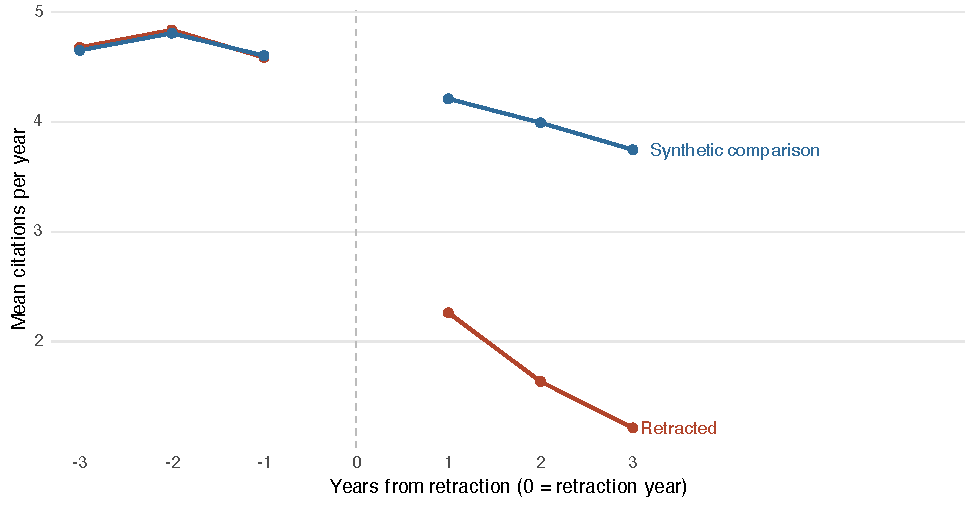
\includegraphics[width=\linewidth]{sdid_paths}
\caption{Mean citations per year to retracted articles and the synthetic comparison path, pooled over cohorts with weights equal to the number of retracted articles.}
\end{figure}

\section{Measurement comparison}
\begin{table}[H]
\centering
\caption{Citations per year to the same articles in the 2016 Web of Science export and in OpenAlex, from each article's publication year through 2015. Ratio is OpenAlex over Web of Science; omitted where Web of Science recorded no citations.}
\adjustbox{max width=\linewidth}{\begin{tabular}{lrrrr}
\toprule
Year & Article-years & Web of Science & OpenAlex & Ratio \\
\midrule
1985 & 1 & 0 & 0 & 1985 \\
1986 & 1 & 0 & 0 & 1986 \\
1987 & 2 & 2 & 1 & 0.50 \\
1988 & 3 & 2 & 1 & 0.50 \\
1989 & 3 & 1 & 0 & 0.00 \\
1990 & 4 & 1 & 2 & 2.00 \\
1991 & 6 & 5 & 5 & 1.00 \\
1992 & 8 & 25 & 25 & 1.00 \\
1993 & 8 & 22 & 17 & 0.77 \\
1994 & 9 & 16 & 8 & 0.50 \\
1995 & 15 & 64 & 55 & 0.86 \\
1996 & 20 & 143 & 109 & 0.76 \\
1997 & 32 & 192 & 143 & 0.74 \\
1998 & 51 & 208 & 190 & 0.91 \\
1999 & 73 & 402 & 377 & 0.94 \\
2000 & 120 & 565 & 585 & 1.03 \\
2001 & 180 & 1,032 & 1,051 & 1.02 \\
2002 & 244 & 1,686 & 1,705 & 1.01 \\
2003 & 317 & 1,835 & 1,907 & 1.04 \\
2004 & 426 & 2,286 & 2,446 & 1.07 \\
2005 & 555 & 2,808 & 3,040 & 1.08 \\
2006 & 728 & 3,326 & 3,605 & 1.08 \\
2007 & 903 & 3,894 & 4,259 & 1.09 \\
2008 & 1,113 & 4,164 & 4,512 & 1.08 \\
2009 & 1,363 & 4,863 & 5,252 & 1.08 \\
2010 & 1,641 & 5,641 & 6,073 & 1.08 \\
2011 & 1,854 & 6,180 & 6,921 & 1.12 \\
2012 & 2,116 & 6,260 & 7,225 & 1.15 \\
2013 & 2,339 & 6,123 & 7,011 & 1.15 \\
2014 & 2,555 & 6,092 & 6,934 & 1.14 \\
2015 & 2,661 & 5,127 & 6,002 & 1.17 \\
\bottomrule
\end{tabular}
}
\end{table}

\section{Retraction rates and timing}
\begin{figure}[H]
\centering
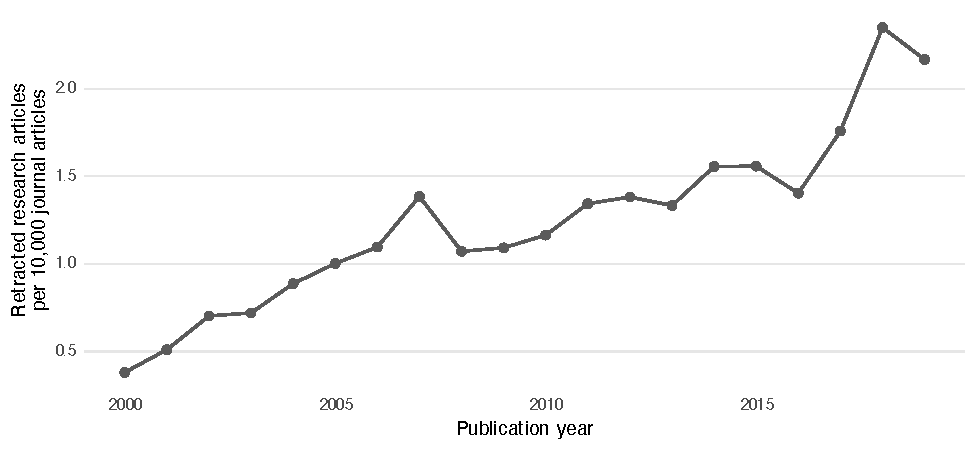
\includegraphics[width=\linewidth]{retraction_rates}
\caption{Frame articles per 10,000 OpenAlex journal articles, by publication year. Later cohorts have had less time to be retracted within the 2005--2022 window.}
\end{figure}
\begin{figure}[H]
\centering
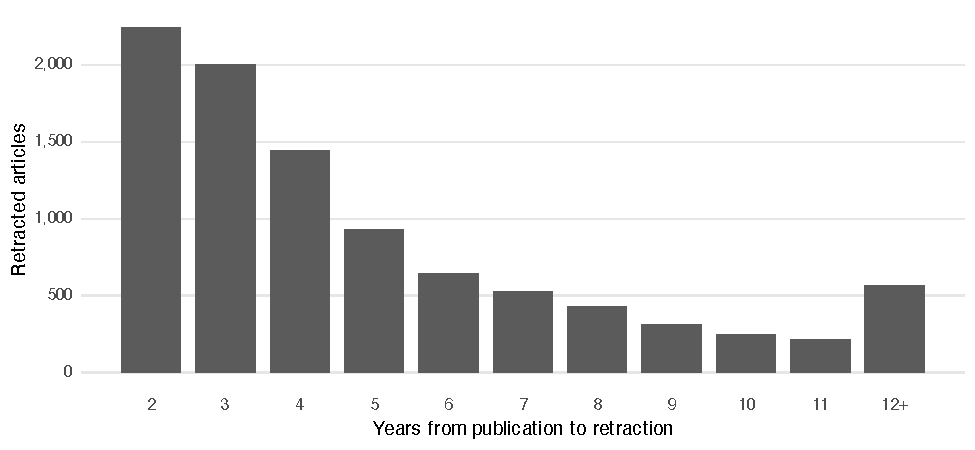
\includegraphics[width=\linewidth]{time_to_retraction}
\caption{Years from publication to retraction for the frame articles.}
\end{figure}
\end{document}
